\documentclass[12pt,a4paper]{report}

\usepackage{styles/dolgozat}
\usepackage{styles/cpp}
\usepackage{styles/python}

\usepackage{listings}
\usepackage{hyperref}
\usepackage{hyphenat}

\usepackage{url,apacite}  

\begin{document}

\pagestyle{empty}

{\large
\begin{center}
\vglue 1truecm
\textbf{\huge\textsc{Szakdolgozat}}\\
\vglue 1truecm

\includegraphics[width=4.8truecm, height=4truecm]{images/me_logo.png}\\
\textbf{\textsc{Miskolci Egyetem}}
\end{center}}

\vglue 1.5truecm

{\LARGE
\begin{center}
\textbf{Rutinszerű feladatok automatizálása grafikus felhasználói felületek esetében}
\end{center}}

\vspace*{2.5truecm}
{\large
\begin{center}
\begin{tabular}{c}
\textbf{Készítette:}\\
Pázmándi Erik\\
Programtervező informatikus
\end{tabular}
\end{center}
\begin{center}
\begin{tabular}{c}
\textbf{Témavezető:}\\
Dr. Kovács Béla
\end{tabular}
\end{center}
\begin{center}
\begin{tabular}{c}
\textbf{Konzulens:}\\
Piller Imre
\end{tabular}
\end{center}}
\vfill

{\large
\begin{center}
\textbf{\textsc{Miskolc, 2022}}
\end{center}}

\newpage


\newpage
\pagestyle{empty}

%Feladatkiiras
\begin{flushleft}
\textsc{\bfseries Miskolci Egyetem}\\
Gépészmérnöki és Informatikai Kar\\
Alkalmazott Matematikai Intézeti Tanszék\hspace*{4cm}\hfil \textbf{Szám:}
\end{flushleft}
\vskip 0.5cm
\begin{center}
\large\textsc{\bfseries Szakdolgozat Feladat}
\end{center}
\vskip 0.5cm
Pázmándi Erik (GXN833) programtervező informatikus jelölt részére.\newline

\noindent\textbf{A szakdolgozat tárgyköre:} Folyamatelemzés, RPA\newline

\noindent\textbf{A szakdolgozat címe:} Rutinszerű feladatok automatizálása grafikus felhasználói felületek esetében\newline

\noindent\textbf{A feladat részletezése:}

\medskip

\emph{A számítógépek kifejlesztésének és használatának egyik fő motivációja, hogy a segít\hyp{}ségével az automatizált módon végrehajtható folyamatok emberi beavatkozás nélkül is végrehajthatóak legyenek. Ennek ellenére számos esetben tapasztalhatjuk, hogy az alkal\hyp{}mazások felhasználói felületén rutinszerűen, repetitíven hajtanak végre műveleteket.}

\medskip

\emph{A dolgozat azt vizsgálja, hogy ezek a folyamatok a korábban rögzített eseménysorok alapján hogyan ismerhetők fel. Bemutatja az RPA (Robotic Process Automation) esz\hyp{}közkészletét, többek között a folyamatelemzés elterjedt módszereit, alkalmazási lehetősé\hyp{}geit, a grafikus felhasználói felületekhez kapcsolódó speciális eseteket. Az elemzésekhez, automatizálást segítő eszköz elkészítéséhez Microsoft Windows platformon Delphi prog\hyp{}ramozási nyelv kerül felhasználásra.}

\vfill

\noindent\textbf{Témavezető:} Dr. Kovács Béla (egyetemi docens) \newline

\noindent\textbf{Konzulens:} Piller Imre (egyetemi tanársegéd) \newline

\noindent\textbf{A feladat kiadásának ideje:} 2021. Szeptember 23.\newline


\vskip 2cm

\hbox to \hsize{\hfil{\hbox to 6cm {\dotfill}\hbox to 1cm{}}}

\hbox to \hsize{\hfil\hbox to 3cm {szakfelelős}\hbox to 2cm{}}

\newpage

\vspace*{1cm}  
\begin{center}
\large\textsc{\bfseries Eredetiségi Nyilatkozat}
\end{center}
\vspace*{2cm}  

Alulírott \textbf{Pázmándi Erik}; Neptun-kód: \texttt{GXN833} a Miskolci Egyetem Gépészmér\hyp{}nöki és Informatikai Karának végzős Programtervező informatikus szakos hallgatója ezennel büntetőjogi és fegyelmi felelősségem tudatában nyilatkozom és aláírásommal igazolom, hogy \textit{Rutinszerű feladatok automatizálása grafikus felhasználói felületek ese\hyp{}tében}
című szakdolgozatom saját, önálló munkám; az abban hivatkozott szakirodalom
felhasználása a forráskezelés szabályai szerint történt.\\

Tudomásul veszem, hogy szakdolgozat esetén plágiumnak számít:
\begin{itemize}
\item szószerinti idézet közlése idézőjel és hivatkozás megjelölése nélkül;
\item tartalmi idézet hivatkozás megjelölése nélkül;
\item más publikált gondolatainak saját gondolatként való feltüntetése.
\end{itemize}

Alulírott kijelentem, hogy a plágium fogalmát megismertem, és tudomásul veszem, hogy
plágium esetén szakdolgozatom visszautasításra kerül.

\vspace*{3cm}

\noindent Miskolc, \hbox to 2cm{\dotfill} .év \hbox to 2cm{\dotfill} .hó \hbox to 2cm{\dotfill} .nap

\vspace*{3cm}

\hspace*{8cm}\begin{tabular}{c}
\hbox to 6cm{\dotfill}\\
Hallgató
\end{tabular}



\newpage

\noindent 1.

\begin{tabular}{cl}
&szükséges (módosítás külön lapon) \\
A szakdolgozat feladat módosítása& \\
& nem szükséges\\
&\\
\hbox to 4cm{\dotfill}&\multicolumn{1}{c}{\hbox to 5cm{\dotfill}}\\
dátum& \multicolumn{1}{c}{témavezető(k)}
\end{tabular}
\vskip1.5mm

\noindent 2. A feladat kidolgozását ellenőriztem:

\vskip1.5mm

\begin{tabular}{l@{\hspace*{4cm}}l}
témavezető (dátum, aláírás):& konzulens (dátum, aláírás):\\
\dotfill&\dotfill\\
\dotfill&\dotfill\\
\dotfill&\dotfill
\end{tabular}

\vskip1.5mm

\noindent 3. A szakdolgozat beadható:

\vskip1.5mm

\begin{tabular}{@{\hspace*{1.3cm}}c@{\hspace*{2.1cm}}c}
\hbox to 4cm{\dotfill}&\multicolumn{1}{c}{\hbox to 5cm{\dotfill}}\\
dátum& \multicolumn{1}{c}{témavezető(k)}
\end{tabular}

\vskip1.5mm

\noindent 4.
\begin{tabular}[t]{@{}l@{\hspace*{1mm}}l@{\hspace*{1mm}}l@{}}
A szakdolgozat& \hbox to 3.5cm{\dotfill} &szövegoldalt\\
              & \hbox to 3.5cm{\dotfill} &program protokollt (listát, felhasználói leírást)\\
              &\hbox to 3.5cm{\dotfill}   &elektronikus adathordozót (részletezve)\\
              &\hbox to 3.5cm{\dotfill} & \\
              &\hbox to 3.5cm{\dotfill} &egyéb mellékletet (részletezve)\\
              &\hbox to 3.5cm{\dotfill} &\\
\end{tabular}
\newline tartalmaz.

\vskip1.5mm

\begin{tabular}{@{\hspace*{1.3cm}}c@{\hspace*{2.1cm}}c}
\hbox to 4cm{\dotfill}&\multicolumn{1}{c}{\hbox to 5cm{\dotfill}}\\
dátum& \multicolumn{1}{c}{témavezető(k)}
\end{tabular}

\noindent 5.

\begin{tabular}{ll}
&bocsátható\\
A szakdolgozat bírálatra& \\
& nem bocsátható\\
\end{tabular}

\vskip1.5mm

\noindent A bíráló neve: \hbox to 8cm{\dotfill}

\vskip4mm

\begin{tabular}{@{\hspace*{1.3cm}}c@{\hspace*{2.1cm}}c}
\hbox to 4cm{\dotfill}&\multicolumn{1}{c}{\hbox to 5cm{\dotfill}}\\
dátum& \multicolumn{1}{c}{szakfelelős}
\end{tabular}

\noindent 6.
\begin{tabular}[t]{@{}l@{\hspace*{1mm}}l@{\hspace*{1mm}}l@{}}
A szakdolgozat osztályzata& &\\
&a témavezető javaslata:& \hbox to 3cm{\dotfill}\\
&a bíráló javaslata:& \hbox to 3cm{\dotfill}\\
&a szakdolgozat végleges eredménye:& \hbox to 3cm{\dotfill}
\end{tabular}

\vspace*{4mm}

\noindent Miskolc, \hbox to 4.5cm{\dotfill} \hspace*{2.5cm}
\begin{tabular}[t]{cc}
\hbox to 6cm{\dotfill}\\
a Záróvizsga Bizottság Elnöke
\end{tabular}


\cleardoublepage
\pagenumbering{gobble}

\tableofcontents

\cleardoublepage
\pagenumbering{arabic}

\newpage

\pagestyle{fancy}

\Chapter{Bevezetés}

Az automatizálás mindig is nagy szerepet játszott az emberiség életében, most pedig az információ korába belépve ez a szerep mégjobban fokozódott mint eddig a történelem során bármikor.

A dolgozat azt vizsgálja, hogy a számítógépek felhasználói felületén miféle sokszor elismételt folyamatok zajlanak le, ezek egy robot szempontjából hogyan is néznek ki, hogyan lehet ezeket utánozni, illetve automatizálni. Bemutatja a Robotikus Folyamat\hyp{}automatizálás (RPA) koncepcióját, annak egy speciális esetét, valamint az ahhoz kötő\hyp{}dő folyamatelemzési modellt.

Bár az RPA mint fogalom annyira már nem új - a 2000-es évek elején bukkant felszínre először -, mégsem annyira elterjedt a köztudatban. Bár sokaknak félelmetes lehet, rengeteg szempontból ezt a technológiát lehet tekinteni az emberi erőforrás gépiesítése felé tett egyik korai lépésnek.

Számos előnnyel rendelkezik a technológia, például olcsóbb egy cég számára mint egy munkavállaló felvétele aki ugyanazokat a tevékenységeket csinálná. Ezen túl megbíz\hyp{}hatóbb is, hiszen az emberi munkással ellentétben nem unatkozik, nem fárad, így a hibalehetőségek aránya eredendően kissebb.
\newline\newline
Ezeken túllépve, a dolgozat inkább egy alacsonyabb szinten tekinti át a technológiát, azaz bemutatja egy gyakorlati implementációját, annak használatát, valamint a felépí\hyp{}tett folyamatokon elvégzett elemzéseket.

Ezzel már egy képet fog kapni az olvasó arról, hogy a legmindennapibb folyamatokat hogyan tudja aránylag rövid időn belül automatizálni, teljes mértékben a saját kényel\hyp{}mének megfelelően.
\Chapter{Koncepció}

\Section{Alpha-algoritmus} 

Az Alpha algoritmus (vagy Alpha bányász) mint folyamatelemzési algoritmus célja, hogy eseménysorozatok halmazából egy ok-okozat rendszert építsen fel. Először van der Aalst, Weijters és Măruşter hozta be a köztudatba. A működésében az eseménysorok halmazát nevezhetjük eseménynaplónak is. Ez az eseménynapló úgynevezett trace hal\hyp{}mazoknak a halmaza, egy trace pedig adott tevékenységnek a sorozata.

Az Alpha bányász volt a legelső folyamatbányászati módszer amit valaha javasoltak és egy egész jó rálátást biztosít a folyamatbányászat céljára, valamint arra, hogy a folyamatokban lévő különböző tevékenységek hogyan is vannak végrehajtva. Emelett, az Alpha bányász szolgált számos újabb folyamatbányászati technika (pl.: Heurisztikus bányász, genetikus bányászat) alapjaként.
	
\begin{definition}{\textit{(Munkafolyamati trace)}} Egy string a $T$ ábécé feladatai közül.\end{definition}
\begin{definition}{\textit{(Munkafolyamati napló)}} Munkafolyamati tracek halmaza.\end{definition}

\subsection{Rövid leírása}	

Az algoritmus egy munkafolyamati naplót $W \subseteq  T^*$ kap bemenetként, és eredményként egy munkafolyamati hálót épít fel.

Ezt az alapján csinálja meg, hogy megvizsgálja az általános kapcsolatokat az egyes feladatok között. Például egy adott feladat lehet, hogy minden esetben megelőz egy másik feladatot, ami egy hasznos információ.

\subsection{Eseménynapló}
Az eseménynapló az elsődleges szükséglet bármely folyamatbányászati algoritmus alkal\hyp{}mazásához. Az eseménynapló a következőket tartalmazza: egyedi azonosító az esethez, tevékenység megnevezése valamint egy időbélyeg. Egy eseménynaplót akár tevékenysé\hyp{}gek halmazának halmazaként is lehet ábrázolni.

Az Alpha bányász szabályai szerint az egyes tevékenységek között az alábbi 4 féle kapcsolat egyike lehetséges:
\begin{enumerate}
\item \textbf{Közvetlen sorrend: $x > y$} akkor és csakis akkor ha az $x$ eseményt közvetlenül követi $y$.
\item \textbf{Okozat: $x \rightarrow y$} ha $x > y$ és nem $y > x$.
\item \textbf{Párhuzam: $x \parallel y$} ha $x > y$ és $y > x$.
\item \textbf{Választás: $x \# y$} ha nem $(x > y)$ és nem $(y > x)$.
\end{enumerate}

\subsection{Minták}

\begin{figure}[h!]
\begin{center}
\caption{\textbf{Szekvencia: A $\rightarrow$ B}}

\includegraphics[width=8truecm, height=4truecm]{images/img_alpha_seq}\\
\label{fig:example}
\end{center}
\end{figure}

\begin{figure}[h!]
\begin{center}
\caption{\textbf{XOR-elágazás: A $\rightarrow$ B, A $\rightarrow$ C} és \textbf{B \# C}}
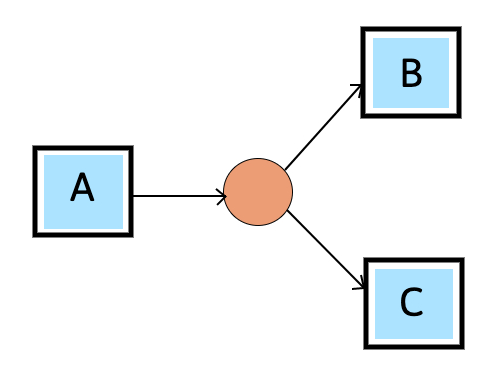
\includegraphics[width=8truecm, height=6truecm]{images/img_alpha_xor}\\
\label{fig:example}
\end{center}
\end{figure}

\begin{figure}[h!]
\begin{center}
\caption{\textbf{ÉS-elágazás: A $\rightarrow$ B, A $\rightarrow$ C} és \textbf{B $\parallel$ C}}
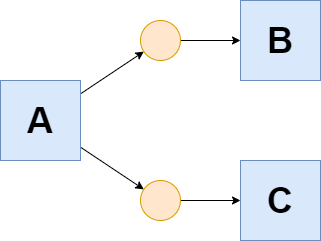
\includegraphics[width=8truecm, height=6truecm]{images/img_alpha_and}\\
\label{fig:example}
\end{center}
\end{figure}

\newpage

\subsection{Példa}
Vegyük példának a következő eseménynaplót:\\
\begin{figure}[h]
\begin{center}
\caption{Példa eseménynaplpó}
\begin{tabular}{||c | c | c ||}
	\hline
	ID & Tevékenység & Időbélyeg \\ [0.5ex]
	\hline\hline
	1 & A & 2022-10-05 13:50:40.000 \\
	\hline
	1 & B & 2022-10-05 16:30:12.000 \\
	\hline
	1 & C & 2022-10-05 16:57:31.000 \\
	\hline
	1 & D & 2022-10-06 13:50:41.000 \\
	\hline
	2 & A & 2022-10-06 15:30:27.000 \\
	\hline
	2 & C & 2022-10-06 16:23:33.000 \\
	\hline
	2 & B & 2022-10-07 08:33:02.000 \\
	\hline
	2 & D & 2022-10-07 12:41:11.000 \\
	\hline
	3 & A & 2022-10-07 13:02:57.000 \\
	\hline
	3 & E & 2022-10-07 14:11:21.000 \\
	\hline
	3 & D & 2022-10-07 14:59:22.000 \\
	\hline
\end{tabular}
\label{fig:example}
\end{center}
\end{figure}\\	
Ebben az esetben az eseménynaplót az alábbi módon tudjuk jelölni:
\[ 
	L_1 = [< A,B,C,D >, <A,C,B,D>, <A,E,D>]
\]

Az Alpha bányász úgy kezdi a munkát, hogy az eseménynaplót közvetlen-sorrend, okozat, párhuzam és választás relációkra alakítja és ezeket felhasználva létrehoz egy petri hálót ami leírja a folyamat modellét.

Első lépésként létrehoz egy lenyomati mátrixot:

\begin{figure}[h!]
\begin{center}
\caption{Példa lenyomati mátrix}
\begin{tabular}{|c | c | c | c | c | c|}
	\hline
	\hspace{0.1cm} & A & B & C & D & E \\
	\hline
	A & \# & $\rightarrow$ & $\rightarrow$ & \# & $\rightarrow$ \\
	\hline
	B & $\leftarrow$ & \# & $\parallel$ & $\rightarrow$ & \# \\
	\hline
	C & $\leftarrow$ & $\parallel$ & \# & $\rightarrow$ & \# \\
	\hline
	D  & \# & $\leftarrow$ & $\leftarrow$ & \# & $\leftarrow$ \\
	\hline
	E & $\leftarrow$ & \# & \# & $\rightarrow$ & \# \\
	\hline
\end{tabular}
\label{fig:example}
\end{center}
\end{figure}

\newpage

\noindent $Y_W$ az összes $(A,B)$  pár halmaza a feladatok maximális halmazából úgy, hogy:
\begin{itemize}
	\item {Egyik $A \times A$ és $B \times B$ sem tagja $>$-nek, és}
	\item {$A \times B$ részhalmaza $\rightarrow$-nek.}
\end{itemize}
\noindent $P_W$ tartalmazza az egyes $Y_W$-hez tartozó helyeket $p_{(A,B)}$, plussz a beviteli $i_W$ helyet és a kimeneti $o_W$ helyet.
\noindent A folyamati reláció $F_W$ az alábbiak uniójából áll össze:
\begin{itemize}
\item $\{(a,p_{(C,B)})|(A,B) \in Y_W \wedge a \in A\}$
\item $\{(p_{(A,B)},b)|(A,B) \in Y_W \wedge b \in B\}$
\item $\{(i_W,t)|t \in T_1\}$
\item $\{(t,i_0)|t \in T_0\}$
\end{itemize}

\noindent Az eredmény

\begin{itemize}
\item egy Petri háló struktúra $\alpha (W) = (P_W, T_W, F_W)$
\item egy beviteli hellyel $i_W$ és egy kimeneti hellyel $o_W$
\item mivel minden $T_W$ átmenet $F_W$-úton van $i_W$-ből $o_W$-be, így valóban egy munka\hyp{}folyamati háló.
\end{itemize}

\noindent Ehhez a példához az alábbi petri háló jön létre az Alpha bányász használatával
\begin{figure}[h]
\caption{Példa kimeneti petri háló}
\begin{center}
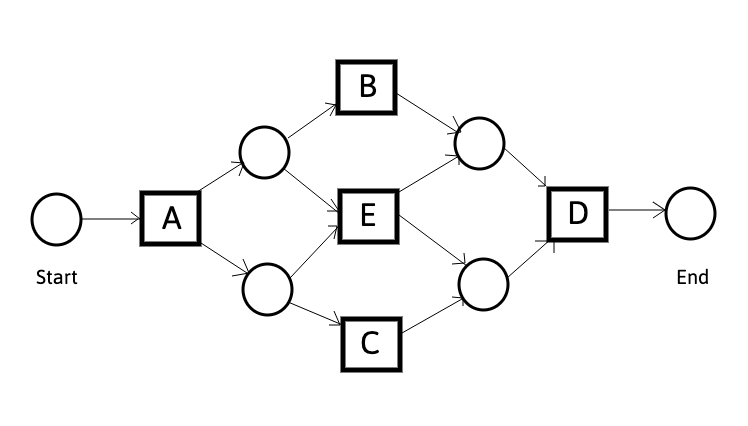
\includegraphics[width=\textwidth,height=\textheight,keepaspectratio]{images/img_alpha_petri_output}\\
\label{fig:example}
\end{center}
\end{figure}

\newpage

\subsection{Korlátozások}
\begin{itemize}
\item \textbf{Implicit helyek}: Az Alpha bányász nem tud különbséget tenni az implicit és a szükséges helyek között, így a felfedezett petri hálóban előfordulhatnak plusz szükségetelen helyek.
\item \textbf{Ciklusok}: Az Alpha bányász nem képes 1-gyes és 2-tes hosszúságú ciklusok felismerésére a folyamatmodellben.
\item A helyi függőségeket gyakran nem veszi észre az Alpha bányász.
\end{itemize}

\textit{Forrás: \cite{wiki:001}}

\Section{Robotic Process Automation} 

A Robotikus Folyamatautomatizálás (továbbiakban: RPA) egy olyan szoftvertechnoló\hyp{}gia, mely lehetővé teszi, hogy az erre specializált szoftverek emberi felhasználót emulál\hyp{}va lépjenek kapcsolatba a számítógépek digitális felületeivel.

Minden egyes ilyen szoftvernek más az eszköztára, van amelyik azt tudja értelmezni, hogy mi van a képernyőn, van amelyik felismer és kinyer adatokat, viszont abban mindegyik osztozik, hogy adott lépésekből meghatározott folyamatokat hajt végre.

Összefoglalva, egy ilyen tökéletesített rendszer ugyanazt tudja mint egy felhasználó, viszont sokkal gyorsabban és konzisztensebben, anélkül, hogy fel kellene állnia nyújtózni vagy elmenni egy kávészünetre.

\subsection{Alkalmazási területek}

Lényegében bármely olyan modern cég tudja hasznosítani ezt a technológiát, mely számítógépet használva pl. nyilvántartást vezet, pénzügyeit digitálisan kezeli, alapvető\hyp{}en a digitális térben mozog, stb..., tehát bárhol ahol embereket digitális tevékenységül alul fel lehet szabadítani.

Elsősorban az adott cégtől függ, hogy belevág-e egy ilyen szoftvertechnológiás meg\hyp{}oldásba, de íme néhány szektor ahol alkalmazható, vagy már alkalmazásra is került:
\begin{itemize}
	\item Egészségügy
	\item Telekommunikáció
	\item Gyártástechnológia
	\item Állami szektor
	\item Kereskedelem
	\item Pénzügyi szolgáltatások
\end{itemize}

Gyakorlatilag csupán az adott folyamattól függ, hogy lebontható-e olyan triviális lépésekre, melyeket már az RPA eszközkészletével automatizálni lehet. Természetesen ahogy fejlődik ez a technológia, úgy egyre nagyobb százalékban lehet majd ezeket is automatizáltnak tekinteni.

Alább található néhány mai rendszer, melyeket a technológia úttörőjének lehet nevezni:
\begin{enumerate}
	\item UIPath
	\item Microsoft Power Automate
	\item Blue Prism
	\item Automaton Anywhere
	\item Kofax
\end{enumerate}

\subsection{A technológia jövője}

Mivel egy automatizációs technológia jövőjéről van szó, ezért az RPA nem egy kis dolog ami feltehetően el fog tűnni, hanem nagy valószínűséggel befolyásolni fogja a munkaerőpiac jövőjének egészét...... (folytatni / elvetni?)

\Section{Delphi}

A dolgozathoz készült szoftver Delphi nyelven íródott, így fontos legalább nagyvona\hyp{}lakban ismerni a nyelvet, hogy tudjuk miért is.

A Delphi egy általános célú erősen típusos objektum orientált programozási nyelv és szoftvertermék ami az Object Pascal programozási nyelv Delphi dialektusát használja, integrált fejlesztői környezetet biztosít, újabban a gyors alkalmazásfejlesztés (RAD, Rapid application development) szoftverfejlesztési elv szerint. A Delphi compilerei natív kódot generálnak a célrendszertől függően, legyen az Microsoft Windows, macOS, iOS, Android vagy Linux (x64).

\textit{\cite{delphi:001}}

\subsection{Múltja röviden}
Az ,,anyanyelve" a Delphinek a Pascal, ami pedig a modellje nagy részét az Algolnak köszönheti - az első magas-szintű progamozási nyelvnek ami olvasható, struktúrált és szisztematikusan meghatározott szintaxissal rendelkezik. A hatvanas években számos utódját fejlesztették az Algolnak, ezek közül a legsikeresebb a Pascal volt.

1983-ban jelent meg az első Turbo Pascal a Borland jóvoltából, ami már integrált fejlesztői környezettel rendelkezett. 1995-ben vezették be a RAD szoftverfejlesztési elvre épülülő környezetet, amit Delphi-nek neveztek, ezáltal átalakítva a Pascal nyelvet egy objektum-orientált vizuális programozási nyelvvé. A célja ennek elsősorban az volt, hogy ennek az új terméknek központi részét képezzék az adatbázis eszközök és kapcsolatok.

2006-ban a Borland átadta a fejlesztőeszközöket a CodeGear nevű leányvállalatá\hyp{}nak, majd ezt a leáanyvállalatot 2008-ban eladta az Embarcadero Technologies-nek. Ez az új cég megtartotta a régi fejlesztői divíziót és számos új verziót dobott piacra. 2015-ben az Idera Software nevű cég pedig felvásárolta az Embarcadero-t és mind a mai napig ugyanúgy Embaracadero márka alatt működteti a fejlesztői eszközök divízióját.

Az évek alatt rendkívül sok modernizáción ment át a Delphi. OLE automatizáció és változó adattípus támogatásától kezdve, DLL debugoláson és XML támogatáson keresztül egészen a multi-platform alkalmazásokig és az in-line változó deklarálásig.

\textit{\cite{delphi:002}}

\subsection{Napjainkban}

Sajnos számos rosszul időzített és rosszul kivitelezett marketing döntés miatt a 2000-es évektől kezdve a Delphi kifejezetten kiesett rengeteg programozó kedvelt programozási nyelve közül, azonban az elmúlt néhány évben ismét sikerült egyre nagyobb ismerettség\hyp{}re szert tennie a komolyabb fejlesztők körében.

Bár közel sem a legelterjedtebb nyelv, számos előnnyel rendelkezik sok másikkal szemben. Ilyenek például az alábbiak:
\begin{enumerate}
	\item \textbf{Könnyen olvasható kód}: Már eredetileg a Pascal megalkotásánál az egyik fő cél az volt, hogy oktatási célra lehessen használni, emberi szemmel is könnyen olvasható legyen a komplex alacsony-szintű kód. Erre egy nagyon jó példa a "\{" és "\}" karakterek (amiket csak a memóriával való spórolás miatt jelöltek így) "begin" és "end" kulcsszóra való cseréje.
	\item \textbf{Multi-platformitás}: A megfelelően megírt (OS-független) kódot néhány kattin\hyp{}tással le lehet fordítani a legismertebb operációs rendszerek natív kódjára.
	\item \textbf{Natív kód}: Az alkalmazás lefordításával natív kódot kapunk, ami azért előny, mert semmilyen egyéb keretrendszer telepítésére nincsen szükségem (pl.: MS C++ Runtime Environment, Java Runtime Environment, stb...)
	\item \textbf{Adatbázis támogatás}: Számos adatbázis kapcsolatot és adatfeldolgozási mód\hyp{}szert beépített módon támogat.
	\item \textbf{Fordítási sebesség}: A mai napig az egyik leggyorsabb a fordítási sebessége más fejlesztőeszközökhöz képest, ezáltal felgyorsíva magát a fejlesztési és debugolási folyamatokat.
\end{enumerate}

\subsection{Delphi a dolgozathoz}

Az előző alfejezetben felsoroltaknak megfelelően kiderült, hogy a Delphi az egy kifeje\hyp{}zetten robosztus és erőteljes programozási nyelv. Ez sok nyelvről elmondható természe\hyp{}tesen, viszont az alábbi két pont miatt került kiválasztásra a dolgozathoz:

\begin{itemize}
	\item \textbf{Modern Windows API}: A fejlesztett szoftver (mint a legtöbb RPA eszköz) közvetlen viszonyban van a Windows API-val, hiszen az operációs rendszer teszi elérhetővé az egyes erőforrásokat (pl. rögzíteni a felhasználó bevitelét még akkor is ha a program háttérben van), illetve teszi lehetővé az input injektálását a folyamat visszajátszásához.
	\item \textbf{Natív kód}: Mivel natív kódra kerül fordításra a programkód, ezért bármely Windows (Vista vagy újabb) operációs rendszerrel rendelkező számítógépen fut\hyp{}tatható a program bármiféle keretrendszer nélkül.
\end{itemize}















\Chapter{Tervezés és Megvalósítás}

A dolgozat által vizsgált témahoz egy komplex multifunkciós szoftver került megterve\hyp{}zésre, mely a dolgozati téma elemzési részében kifejezetten nagy szerepet tölt be. Összetettsége révén rengeteg időt és odafigyelést igényelt már maga a tervezési fázis is. Számos ábra és tervezet került megalkotásra, melynek a túlnyomó része rendkívül jelentősnek bizonyult az implementáció során.

\Section{Dizájn}

A legmagasabb szinten az alábbi ábra nyújtja a legtisztább áttekintését a különböző funkcióknak és a szoftver sokszínűségének.

\begin{figure}[h!]
\begin{center}
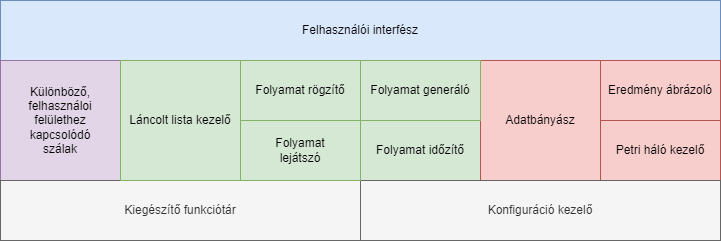
\includegraphics[width=\textwidth,keepaspectratio=true]{images/img_plan_1}
\caption{\textbf{High-level áttekintő ábra}}
\label{fig:plan}
\end{center}
\end{figure}

\begin{itemize}
	\item \textbf{Felhasználói interfész}: A kezelőfelület, amivel a felhasználó eléri és kezelni tudja az egyes szoftverfunkciókat.
	\item \textbf{Felhasználói felülethez kapcsolódó szálak}: Fontos - a felhasználó számára nem látható - szálak, amelyek feldata bizonyos billentyűkombinációk figyelése anélkül, hogy a program reszponzivitását kártékonyan befolyásolnák.
	\item \textbf{Láncolt lista kezelő}: Az egyes folyamatok láncolt listaként vannak kezelve a szoftverbe, ez az alrendszer felel a megfelelő értelmezésükért. 
	\item \textbf{Folyamat rögzítő}: Figyeli és rögzíti a perifériák általi beviteli értékeket.
	\item \textbf{Folymat generáló}: Előre meghatározott forgatóvkönyvek alapján úgy generál folyamatokat mintha azt egy felhasználó végezte volna el.
	\item \textbf{Folyamat lejátszó}: A folyamatokat játsza vissza, egy felhasználót szimulál.
	\item \textbf{Folyamat időzítő}: A Windowsba integrált rendszert felhasználva ütemez / időzít folyamatokat.
	\item \textbf{Adatbányász}: Az Alpha-algoritmust implementálva folyamatelemzést hajt végre több folyamaton.
	\item \textbf{Eredmény ábrázoló}: Az Adatbányász által elvégzett folyamatelemzés eredmé\hyp{}nyeit jeleníti meg.
	\item \textbf{Petri-háló kezelő}: A Petri-hálót mint struktúra, valamint a hozzátartozó függ\hyp{}vényeket a szoftver számára értelmezhető módon implementálja.
	\item \textbf{Kiegészítő funkciótár}: Számos hasznos funkció gyűjteménye, melyet a többi alrendsze használ.
	\item \textbf{Konfiguráció kezelő}: Futásidők között felhasználói preferenciák és beállítások tárolásáért és betöltéséért felel.
\end{itemize}

\Section{Folyamatelemzés}

Az Alpha-algoritmust mint folyamatelemzési módszert hasznosan lehet alkalmazni a dolgozati témában. Az algoritmus, jelentőségét tekintve elengedhetetlen részét képezi a dolgozatnak. Jelen esetben a folyamatokat azok jellegétől és céljától függetlenül lehet elemezni, akár cél nélküli beviteli sorozatra is alkalmazható az Alpha-algoritmus.

\subsection{Az Alpha-algoritmus}

Ebben az alfejezetben bemutatásra kerül, hogy hogyan is kapcsolódik pontosan az Alpha-algoritmus a dolgozat témájához.

Először is pontosan meg kell határozni, hogy milyen lépésekből áll az algoritmus.

\begin{definition}{\textit{($\alpha$-algoritmus):}} Legyen $L$ egy eseménynapló adott $E$ események hal\hyp{}maza felett. Ekkor a kimeneti $\alpha (L)$ Petri-hálót az alábbi módon határozzuk meg:
\begin{enumerate}
	\item Definiáljuk az összes eseményt.\\
	\[
		E_L = \{ e \in E | \exists_{\sigma \in L} e \in \sigma \},
	\]
	\item Definiáljuk az összes bemeneti eseményt.
	\[
		E_I = \{ e \in E | \exists_{\sigma \in L} e = first(\sigma) \},
	\]
	\item Definiáljuk az összes kimeneti eseményt.
	\[
		E_O = \{ e \in E | \exists_{\sigma \in L} e = last(\sigma) \},	
	\]
	\item Kiszámítjuk az összes lehetséges $A$ és $B$ halmazt úgy, hogy az összes esemény $A$-ban és $B$-ben függetlenek legyenek egymástól, valamint minden $A$-beli esemény okozati kapcsolatban álljon $B$-beli eseményekhez.
	\begin{equation*}
	\begin{aligned}
		X_L=
		&\{ (A,B) | A \subseteq E_L \land A \neq \emptyset \land B \subseteq E_L \land B \neq \emptyset \land \\
		&\forall_{a \in A} \forall_{b \in B} a \rightarrow_L b \land \forall_{a1,a2 \in A} a_1\#_L a_2  \land \forall_{b1,b2 \in B} b_1\#_Lb_2\},
	\end{aligned}
	\end{equation*}
	\item Elhagyjuk a nem-maxmiális halmazokat.
	\[
		Y_L = \{ (A,B) \in X_L | \forall_{A',B' \in X_L} A \subseteq A' \land B \subseteq B' \Rightarrow (A,B) = (A',B') \},
	\]
	\item Helyeket rendelünk az összes származtatott halmazhoz valamint a kezdő- és végál\hyp{}lapotokhoz.
	\[
		P_L = \{ p_{A,B} | (A,B) \in Y_L\} \cup \{i_L,o_L\},		
	\]
	\item Berajzoljuk a kapcsolatokat.
	\begin{equation*}
	\begin{aligned}
		F_L=
		&\{(a,p_{(A,B)} | (A,B) \in Y_L \land a \in A \} \cup \{ (p_{(A,B)}, b) | (A,B) \in \\
		&Y_L \land b \in B \} \cup \{ (i_L,e) | e \in E_I \} \cup \{ (e,o_L) | e \in E_O\},
	\end{aligned}
	\end{equation*}
	\item Visszatérünk a Petri-hálóval.
	\[
		\alpha(L) = (P_L, E_L, F_L).
	\]

\end{enumerate}

\cite{article:001}
\end{definition}

\begin{example}
	Itt három előre létrehozott folyamaton kerül alkalmazásra az algoritmus. A folyamatok egyszerűek, hogy szemléletes legyen a példa, viszont ugyanezzel a mód\hyp{}szerrel több száz vagy akár több ezer hosszú folyamaton is alkalmazható az algoritmus.
	
	Maguk a folyamatok szolgálnak bemenetként, részeredményekként eseménynapló és lenyomati mátrix jön létre, kimentként pedig egy olyan Petri-háló kerül generálásra mely leírja a folyamat modelljét.

	Vegyük az alábbi táblázatot.
	\newpage

	\begin{table}[h!]
	\begin{center}
	\caption{Beviteli folyamatok}
	\begin{tabular}{|| c | c | c | c | c | r ||}
		\hline\hline
		\textbf{Folyamat} & \textbf{ID} & \textbf{Típus} & \textbf{Érték} & \textbf{Érték típusa} &  \textbf{Eltelt idő} \\ [0.5ex]
		\hline\hline
		1 & 1 & Key&  Left Alt & WM\_SYSKEYDOWN & 0 \\
		\hline
		1 & 2 & Key&  F4 & WM\_SYSKEYDOWN & 100 \\
		\hline
		1 & 3 & Key&  F4 & WM\_SYSKEYUP & 150 \\
		\hline
		1 & 4 & Key&  Left Alt & WM\_KEYUP & 612 \\
		\hline\hline
		2 & 1 & Key & Left Alt & WM\_SYSKEYDOWN & 0 \\
		\hline
		2 & 2 & Key & F4 & WM\_SYSKEYUP & 80 \\
		\hline
		2 & 3 & Key & F4 & WM\_SYSKEYDOWN & 51 \\
		\hline
		2 & 4 & Key & Left Alt & WM\_KEYUP & 152 \\
		\hline\hline
		3 & 1 & Key & Left Alt & WM\_SYSKEYDOWN & 0 \\
		\hline
		3 & 2 & Mouse & 25:1022 & WM\_LBUTTONDOWN & 151 \\
		\hline
		3 & 3 & Key & Left Alt & WM\_KEYUP & 188 \\
		\hline\hline
	\end{tabular}
	\label{fig:planexample}
	\end{center}
	\end{table}	

	Az Alpha-algoritmus alkalmazásában, mint bármely folyamatbányászati algorit\hyp{}musnál, első lépésként ezekből az eseményekből fel kell építeni az eseménynaplót amiből később dolgozik az algoritmus. Ez a lépés konkrétan arról szól, hogy a már meglévő folyamatok az Alpha-algoritmusnak szükséges formátumra kerülnek átalakításra.
	
	Ez jelen esetben az alábbi három szabály alapján történik:
	\begin{enumerate}
		\item A "\textbf{Folyamat}" elnevezésű oszlop alapján triviális módon meghatározásra kerül az esethez tartozó egyedi azonosító,
		\item A "\textbf{Típus}", "\textbf{Érték}" és "\textbf{Érték típusa}" oszlophármas értékeiből létrejön a tevékenység megnevezése,  ami a továbbiakban \textit{,,$T_{n}$"}-ként lesz feltüntet\hyp{}ve,
		\item Az "\textbf{Eltelt idő}" oszlop alapján (az előző esemény óta eltelt időt mutatja) pedig létrejön egy relatív-időbélyeg az "\textbf{ID}" oszlop segítségével, hiszen az utóbbi alap\hyp{}ján határozható meg az események szekvenciája.
	\end{enumerate}
	
	Ezeknek megfelelően az alábbi eseménynaplót kapjuk:
	\newpage

	\begin{table}[h]
	\begin{center}
	\caption{Eseménynapló}
	\begin{tabular}{|| c | c | c ||}
		\hline
		Azonosító & Tevékenység & Relatív időbélyeg \\ [0.5ex]
		\hline\hline
		1 & $T_0$ & 0 \\
		\hline
		1 & $T_1$ & 100 \\
		\hline
		1 & $T_2$ & 250 \\
		\hline
		1 & $T_3$ & 762 \\
		\hline
		2 & $T_0$ & 0 \\
		\hline
		2 & $T_2$ & 80 \\
		\hline
		2 & $T_1$ & 131 \\
		\hline
		2 & $T_3$ & 283 \\
		\hline
		3 & $T_0$ & 0 \\
		\hline
		3 & $T_4$ & 151 \\
		\hline
		3 & $T_3$ & 339 \\
		\hline
	\end{tabular}
	\label{fig:planexample}
	\end{center}
	\end{table}	
	
	Miután megvan az eseménynapló, a következő két lépésben meghatározzuk a beme\hyp{}neti- és kimeneti események halmazait:
	\begin{enumerate}
		\item $E_I=<T_0>$
		\item $E_O=<T_3>$		
	\end{enumerate}

	Ezután a következő lépéshez az eseménynaplóban szereplő események kapcsolatait közvetlen-sorrend, okozat, párhuzam és választás relációkra alakítja az algoritmus.

	Ezzel jön létre az alábbi lenyomati mátrix:
	
	\begin{table}[h]
	\begin{center}
	\caption{Lenyomati mátrix}
	\begin{tabular}{|c | c | c | c | c | c|}
		\hline
		\hspace{0.1cm} & $T_0$ & $T_1$ & $T_2$ & $T_3$ & $T_4$ \\
		\hline
		$T_0$ & \# & $\rightarrow$ & $\rightarrow$ & \# & $\rightarrow$ \\
		\hline
		$T_1$ & $\leftarrow$ & \# & $\parallel$ & $\rightarrow$ & \# \\
		\hline
		$T_2$ & $\leftarrow$ & $\parallel$ & \# & $\rightarrow$ & \# \\
		\hline
		$T_3$ & \# & $\leftarrow$ & $\leftarrow$ & \# & $\leftarrow$ \\
		\hline
		$T_4$ & $\leftarrow$ & \# & \# & $\rightarrow$ & \# \\
		\hline
	\end{tabular}
	\label{fig:planexample}
	\end{center}
	\end{table}

	Ezen a mátrixon kerül ábrázolásra az összes esemény közötti kapcsolat. Több szem\hyp{}pontból is hasznos ez a mátrix, többek között a struktúrája is megfelelő ahhoz, hogy program szinten meghatározzuk a következő lépésben a lehetséges halmazpárokat, vala\hyp{}mint emberi szemmel is kifejezetten könnyen értelmezhető.

	Ezt a mátrixot felhasználva az alábbi halmazpárok lehetségesek a jelenlegi példában:
	\newpage

	\begin{table}[h]
	\begin{center}
	\caption{Lehetséges halmazpárok}
	\begin{tabular}{|| c | c ||}
		\hline
		A & B \\
		\hline\hline
		\{$T_0$\} & \{$T_1$\} \\
		\hline
		\{$T_0$\} & \{$T_2$\} \\
		\hline
		\{$T_0$\} & \{$T_4$\} \\
		\hline
		\{$T_1$\} & \{$T_3$\} \\
		\hline
		\{$T_2$\} & \{$T_3$\} \\
		\hline
		\{$T_4$\} & \{$T_3$\} \\
		\hline
		\{$T_0$\} & \{$T_1, T_4$\} \\
		\hline
		\{$T_0$\} & \{$T_2, T_4$\} \\
		\hline
		\{$T_1, T_4$\} & \{$T_3$\} \\
		\hline
		\{$T_2, T_4$\} & \{$T_3$\} \\
		\hline
	\end{tabular}
	\label{fig:planexample}
	\end{center}
	\end{table}	

	Következő lépésként ezekből a halmazpárokból kell eltávolítani a nem-maximálisak\hyp{}at, azaz azokat amik részhalmazai egy másiknak. Ezt program szinten egy többszörös ciklus segítségével könnyedén el lehet végezni, jelen példában pedig az alábbi négy halmazpár maradt:
	
	\begin{table}[h]
	\begin{center}
	\caption{Maradék halmazpárok}
	\begin{tabular}{|| c | c ||}
		\hline
		A & B \\
		\hline\hline
		\{$T_0$\} & \{$T_1, T_4$\} \\
		\hline
		\{$T_0$\} & \{$T_2, T_4$\} \\
		\hline
		\{$T_1, T_4$\} & \{$T_3$\} \\
		\hline
		\{$T_2, T_4$\} & \{$T_3$\} \\
		\hline
	\end{tabular}
	\label{fig:planexample}
	\end{center}
	\end{table}

	Miután ezek a halmazpárok meghatározásra kerültek, helyek $(p_1-p_4)$  lesznek hozzájuk rendelve. Ezekhez a helyekhez létrehozásra kerülnek a megfelelő bemeneti és kimeneti átmenetek, valamint a végső bemeneti és kimeneti állapotok is.

	Amint ez megvan, berajzolásra kerülnek a kapcsolatok is, a végén pedig a következő Petri-háló kerül megjelenítésre.
	\newpage

	\begin{figure}[h!]
	\begin{center}
	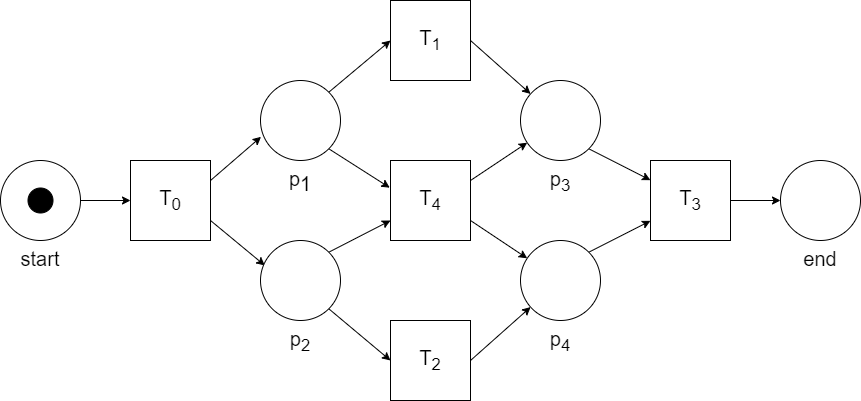
\includegraphics[width=\textwidth,keepaspectratio=true]{images/img_plan_2}
	\caption{Kimeneti Petri-háló}
	\label{fig:plan}
	\end{center}
	\end{figure}


\end{example}

\definecolor{codeComment}{RGB}{0, 128, 0}
\definecolor{codeKeyword}{RGB}{0, 0, 255}
\definecolor{codeNumber}{RGB}{100, 100, 255}
\definecolor{codeString}{RGB}{100, 100, 255}
\lstdefinestyle{delphicode}{
	language=Delphi, 
	commentstyle=\color{codeComment},
	keywordstyle=\color{codeKeyword},
	numberstyle=\tiny\color{codeNumber},
	stringstyle=\color{codeString},
	basicstyle=\ttfamily\footnotesize,
	breaklines=true,
	showspaces=false,
	showstringspaces=false
}
\lstset{style=delphicode}


\Section{Implementáció}

A program gyakorlati megvalósítása egy-két apróságtól eltekintve megegyezik a terve\hyp{}zettel. Az alapvető stuktúrát megtartotta, az egymáshoz tartozó funkciók, változók és kódrészletek külön egységekbe (továbbiakban: unitok) lettek szervezve, így csoportosít\hyp{}va az egyes szoftverfunkciókat.

Ezek a unitok többféle kapcsolatban állhatnak egymással, az egymásra való hivatko\hyp{}zásuknak függvényében. Ezeket a kapcsolatokat a 3.3 ábra demonstrálja.

\begin{figure}[h]
	\begin{center}
		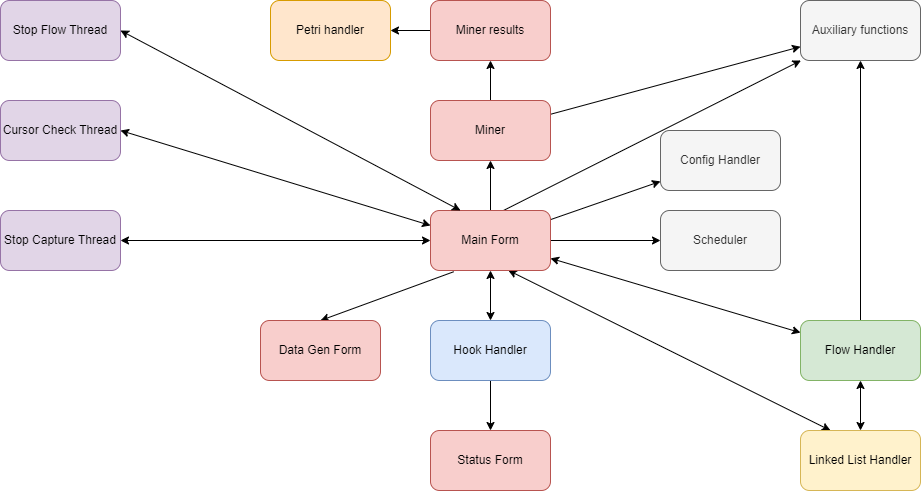
\includegraphics[width=0.95\textwidth, keepaspectratio=true]{images/unitok_kapcsolati_abra}\\
		\label{fig:example}
	\end{center}
	\caption{Unitok kapcsolatai}
\end{figure}

Pirossal azok a unitok láthatók melyekhez tartozik grafikus felület is, a további színek pedig az egyes funkciók csoportosítására szolgálnak. Részletesebben a unitokról a következő pontokban olvashatunk.

\begin{itemize}
	\item{
		\textbf{Unit\_Main}: Ez a program főegysége, ebben került implementálásra a főablak és annak felhasználói felülete. Az alábbi feladatokat látja el.
		\begin{enumerate}
			\item{Implementálja a felhasználói felület objektumait, azoknak a tulajdonságait és rutinjait.}
			\item{Inicializálja a programot futtatásnál, betölti a felhasználó konfigurációit.}
			\item{Kezeli a program rendszertálcára való kicsinyítését.}
			\item{Kezeli azt a néhány globális változót amik szükségesek (pl.: a futtatható fájl elérési útvonala).}			
		\end{enumerate}
	}
	\item{
		\textbf{Unit\_ConfigHandler}: A konfigurációkezelő osztályt, az abba tartozó objek\hyp{}tumokat és rutinokat implementálja, melyek lehetővé teszik a futásidő alatti konfigurációs beállítások titkosítva történő tárolását.
		\begin{lstlisting}
  TConfigHandler = class(TObject)
    configFile: string;
    configArray: array of array of string;

  public
    procedure Save(Key: string; Value: string);
    function Load(Key: string; Fallback: string): string;

    constructor Create(filePath: string);
    destructor Destroy; override;

    function Encrypt(const value: string): UnicodeString;
    function Decrypt(const value: string): UnicodeString;

    function MatchCharToArrayIndex(const character: char): integer;
  end;
		\end{lstlisting}
	}
	\item{
		\textbf{Unit\_AuxiliaryFunctions}: Néhány olyan kiegészítő rutint tartalmazó gyűjte\hyp{}mény, melyeket a többi egység használ. Külön egységbe ki lettek gyűjtve, hogy az OOP alapelvek teljesüljenek.
	}
	\item{
		\textbf{Unit\_StopFlowThread}: Egy olyan szálat implementáló egység, amely feladata kifejezetten a \textbf{F2 + F3} billentyűkombináció lenyomásának felügyelete.

		Ez a billentyűkombináció felel azért, hogy az éppen futó folyamatot le lehessen futás közben állítani. Feltétlenül szükséges, hogy ez ilyen módon legyen implemen\hyp{}tálva, hiszen ennek a billentyűkombinációnak akkor is működnie kell, ha a fókusz éppen egy másik alkalmazáson van.

A Windows API és a \textbf{Unit\_Main} által implementált rutinokra és változókra hivatkozik a műküdése során.
		\begin{lstlisting}
procedure TStopFlowThread.Execute;
begin
  repeat
    if (GetKeyState(VK_F2) < 0) and (GetKeyState(VK_F3) < 0) then
    begin
      Form1.Btn_StartFlowClick(stopFlowThread);
    end;
  until not runStopFlow;
end;
		\end{lstlisting}
	}
	\item{
		\textbf{Unit\_CursorCheckThread}: Egy olyan szálat implementáló egység, melynek feladata a kurzor aktuális pozíciójának a felhasználói felületen történő frissítése. Windows API-t meghívva jut hozzá a szükséges adathoz.
		\begin{lstlisting}
procedure TCursorCheckThread.Execute;
var
  p: TPoint;
begin
  FreeOnTerminate := true;
  repeat
    GetCursorPos(p);
    Form1.Lab_Cursor_X.Caption := 'x: ' + IntToStr(p.X);
    Form1.Lab_Cursor_Y.Caption := 'y: ' + IntToStr(p.Y);
  until not runCursorPos;
end;
		\end{lstlisting}
		Ennek a célja, az, hogy amikor a felhasználó kézileg akar egérkattintást hozzáadni az aktuális folyamathoz, akkor megkönnyítse a megfelelő képernyő-koordináták meghatározását.
	}
	\item{
		\textbf{Unit\_StopCaptureThread}: Egy olyan szálat implementáló egység, melynek feladata hasonló az előzőekben bemutatott \textbf{TStopFlowThread}-éhez.

Az eltérés annyi, hogy az \textbf{F2 + F4} billentyűkombinációt figyeli, melynek lenyo\hyp{}mására egy olyan rutint hív meg, mely leállítja az éppen futó felhasználói ese\hyp{}ménysor rögzítését.
	}
	\item{
		\textbf{Unit\_LinkedListHandler}: Egy olyan struktúrát implementál, melyre a szoft\hyp{}ver összes többi folyamatkezezlő egysége épül. Az ebből a láncolt lista struktúrá\hyp{}ból példányosított elemek tartalmazzák a folyamat lépéseihez tartozó összes infor\hyp{}mációt.

	Először is implementál két felsorolás típust, melyek intuitív módon leírják magu\hyp{}kat:
	\begin{lstlisting}
type
  // Enum
  TInputType = (itClick, itKeyboard, itSpecialKey, itHotkey);
  TWaitType = (wtMil, wtSec, wtMin, wtHour);
	\end{lstlisting}

	valamint definiálja a láncolt lista elemet és az arra hivatkozó mutatót:
	\begin{lstlisting}
  // Linked List pointer type
  PFlowElement = ^TFlowElement;

  // Linked List element
  TFlowElement = record
    inputType: TInputType;
    inputParam1: string;
    inputParam2: string;
    inputParam3: string;
    inputParam4: string;
    waitAfterAmount: integer;
    waitAfterType: TWaitType;
    waitAfterTypeText: string;
    deleteButton: TButton;
    panelObject: TPanel;
    labelObject: TLabel;
    NextElement: PFlowElement;
  end;
	\end{lstlisting}

	Ezek mellett még tartalmaz egy rutint, mely arra szolgál, hogy egy meglévő láncolt lista elemtől kezdve az összes további elemhez tartozó objektumot megfele\hyp{}lően szabadítsa fel a memóriából.

	}
	\item{
		\textbf{Unit\_FlowHandler}: A folyamatokhoz tartozó legfontosabb rutinokat definiál\hyp{}ja, amik a következőek:
		\begin{enumerate}
			\item{folyamat mentése fájlba,}
			\item{folyamat betöltése állományból,}
			\item{folyamat generálása a felhasználói bevitelből rögzített eseméysorból,}
			\item{adott folyamati lépés végrehajtása, azaz input injektálása a Windows felé. pl.:
				\begin{lstlisting}
if (currentStep.inputParam3 = 'Left') and
(currentStep.inputParam4 = 'Down+Up (single)') then
begin
  mouse_event(MOUSEEVENTF_LEFTDOWN, 0, 0, 0, 0);
  mouse_event(MOUSEEVENTF_LEFTUP, 0, 0, 0, 0);
end 
				\end{lstlisting}
			} 
			
		\end{enumerate}
	}
	\item{
		\textbf{Unit\_HookHandler}: Ennek az egységnek a feladata azoknak az objektumok\hyp{}nak, változóknak és függvényeknek az implementációja, melyek lehetővé teszik a felhasználói input rögzítését a Windows API \textit{hook}-jainak felhasználásával.

A \textit{hook} egy olyan pont a rendszer üzenetkezelő mechanizmusában, ahová a szoft\hyp{}ver egy olyan szubrutint telepít, mely figyeli az üzenet forgalmat a rendszerben, és feldolgozza azokat még mielőtt elérné a cél-ablakhoz tartozó eljárását.

A felhasználói input rözítésénél két ilyen \textit{hook} kerül telepítésre: egy a billentyűzet üzenetsornak, a másik pedig az egérhez tartozóhoz. Ezek a telepítések a Win\hyp{}dows API által biztosított
\begin{lstlisting}
function SetWindowsHookEx; external user32 name 'SetWindowsHookExW';
\end{lstlisting}
függvény hívásával történnek.

Ezeken túl az egység tartalmaz egy olyan funkciót is, mely az adott konstanst (vagy karakterkódot) ember által könnyen értelmezhető szövegre fordítja, pl. \textbf{VK\_PRIOR} $\rightarrow$ \textbf{[Page Up]}, vagy \textbf{65} $\rightarrow$ \textbf{[a]}

	}
	\item{
		\textbf{Unit\_Status}: Ez az egység azt az ablakot implementálja, mely visszajelzést ad az éppen futó eseménysor-rögzítés lépéseiről.
		\begin{lstlisting}
type
  TForm_Status = class(TForm)
    Lab_Input: TLabel;
    Lab_Finish: TLabel;
    Lab_Input_Title: TLabel;
    Lab_StepID_Title: TLabel;
    Pnl_Main: TPanel;
    Lab_StepID: TLabel;
    procedure FormCreate(Sender: TObject);
    procedure FormShow(Sender: TObject);
    procedure FormMouseMove(Sender: TObject; Shift: TShiftState; X, Y: Integer);
  public
    procedure UpdateLabel_Input(newText: string);
    procedure UpdateLabel_StepID(newID: integer);
  end;
		\end{lstlisting}

A rutinjai lehetővé teszik, hogy más egységből (pl.:\textbf{Unit\_HookHandler}) is lehes\hyp{}sen frissíteni a grafikus elemeit, valamint, hogy folyamatrögzítés közben hiába látszik az ablak, akkor se legyen útban a felhasználónak.
	}
	\item{
		\textbf{Unit\_Scheduler}: Két egyszerű függvényt implementáló osztályt definiál, mely arra szolgál, hogy a Windows API segítségével meghívott \textit{schtasks.exe} feladatüte\hyp{}mezőbe rögzíteni, illetve onnan törölni lehessen folyamatokat.
	\begin{lstlisting}
  TScheduleHandler = class(TObject)
  public
    function DeleteTask(fPath: string): integer;
    function AddTask(fPath, sPath: string): integer;
  end;
	\end{lstlisting}
	}
	\item{
		\textbf{Unit\_DataGenerator}: Egy felületet és számos rutint definiál, melyek segítsé\hyp{}gével könnyedén folyamatokat lehet generálni. Ennek az a célja, hogy az adatbá\hyp{}nyászathoz elegendő mennyiségű folyamatot lehessen meghatározni emberi időn belül.

	\begin{lstlisting}
type
  TForm_Generator = class(TForm)
    Mem_Log: TMemo;
    Pnl_Interface: TPanel;
    Btn_Generate: TButton;
    RadGroup_GenCategory: TRadioGroup;
    Spin_GenCount: TSpinEdit;
    procedure Btn_GenerateClick(Sender: TObject);
    procedure FormCloseQuery(Sender: TObject;
    var CanClose: Boolean);
  private
    { Private declarations }
    procedure Generate_ComputerShutdown(count: integer);
    procedure Generate_ComputerRestart(count: integer);
    procedure Generate_BrowserLaunch(count: integer);
    procedure AddToLog(msg: string);

    function GetClickDelay(_type: integer): integer;
    function GetRandomMouseCoordinate(min, max: integer):integer;
  end;

	\end{lstlisting}

		Három forgatókönyv került létrehozásra, ezekből választva lehetséges a generálás. A feladatot elvégezve a folyamatokat egy adott mappába állományonként menti le a szoftver.
	}
	\item{
		\textbf{Unit\_Miner}: Egy felület ami az Alpha-algoritmust illetve a Heurisztikus Bá\hyp{}nyászt  implementálja. A felületet használva a bányászat megkezdését követően láthatjuk, hogy éppen hol jár a választott algoritmustban a szoftver.
	\begin{lstlisting}
type
  TForm_Miner = class(TForm)
    Panel_Interface: TPanel;
    Mem_Log: TMemo;
    Edt_DataPath: TEdit;
    Pnl_DataPath: TPanel;
    Lab_DataPath: TLabel;
    Btn_DataPath_Browse: TButton;
    Btn_Begin: TButton;
    procedure FormCloseQuery(Sender: TObject;
    var CanClose: Boolean);
    procedure Btn_DataPath_BrowseClick(Sender: TObject);
    procedure Btn_BeginClick(Sender: TObject);
  private
    procedure AddToLog(msg: string);
    procedure AlphaMine();
    procedure ChangeUserControl(newState: boolean);
    function RemoveBracketsFromString(str: string): string;
    function IsInActivityList(str: string): boolean;
    function GetNewActivityID: string;
    function FindActivityID(str: string): string;
  end;
	\end{lstlisting}

Amint végzett az algoritmus, az eredményeket a következő \textbf{Unit\_MinerResults} által definiált ablakban ábrázolja.

A halmazpárok három-dimenziós adatstruktúrában vannak tárolva, illetve kezel\hyp{}ve. Ezeknek az értelmezése elég komoly odafigyelést igényel.
	\begin{lstlisting}
  TArrayOfSets = array of array of array of integer;
	\end{lstlisting}

	}
	\item{
		\textbf{Unit\_MinerResults}: Azt a felületet implementáló egység, mely a választott bányász eredményeit jeleníti meg grafikusan. Ezek:
		\begin{enumerate}
			\item{a létrejött eseménynapló,}
			\item{az eseménynaplóbó létrejött lenyomati mátrix (Heurisztikus bányásznál füg\hyp{}gőségi mátrix),}
			\item{az összes maximális halmaz (Alpha-algoritmus esetében),}
			\item{a kimeneti Petri-háló, melyet a \textbf{Unit\_PetriHandler} segítségével generál.}
		\end{enumerate}
		\begin{lstlisting}
  TForm_MinerResults = class(TForm)
  .
  .
  .
  public
    procedure DrawPetriNet(arrayOfSets: TArrayOfSets);
    procedure DrawPlace(startX, startY: integer; lab: string);
    procedure DrawTransition(startX, startY: integer; lab: string);

    procedure DrawArrow(startX, startY, endX, endY: integer); overload;
    procedure DrawArrow(endX, endY: integer); overload;

    function GetStartEvents(): TIntegerArray;
    function GetEndEvents(): TIntegerArray;
  end;

		\end{lstlisting}
	}
	\item{
		\textbf{Unit\_PetriHandler}: Számos objektumot és rutint implementál, melyek segít\hyp{}ségével felépíthető és megjeleníthető egy Petri-háló.
		\begin{enumerate}
			\item{Definiálja a helyeket,
				\begin{lstlisting}
  TPetriPlace = record
    name: string;
    fromList: TStringArray;
    toList: TStringArray;
    location: TPoint;
    recursionLock: boolean;
  end;
				\end{lstlisting}
			}
			\item{Definiálja az átmeneteket,
				\begin{lstlisting}
  TPetriTransition = record
    id: integer;
    fromList: TStringArray;
    toList: TStringArray;
    location: TPoint;
    recursionLock: boolean;
  end;
				\end{lstlisting}
			}
			\item{Definiál egy Petri-háló gyűjteményt, melyben tárolni lehet a helyeket és átmeneteket, valamint a rutinok segítségével fel lehet térképezni a közöttük lévő kapcsolatokat.
				\begin{lstlisting}
  TPetriCollection = class(TObject)
    places: array of TPetriPlace;
    transitions: array of TPetriTransition;
    objectSize: integer;
  public
    constructor Create();
    destructor Destroy(); override;
    procedure NewPlace(_name: string; _fromList, _toList: TStringArray);
    procedure NewTransition(_id: integer; _fromList, _toList: TStringArray);
    function FindIndexOfPlace(name: string): integer;
    function FindIndexOfTransition(id: integer): integer;
    procedure MapTransitions();
    procedure MapPlaceLocation(currentTransition: TPetriTransition);
    procedure MapTransitionLocation(currentPlace: TPetriPlace);
    procedure UpdateList(var list: TStringArray; newValue: string);
    function GetMaxIndexInColumn(col: integer): integer;
  end;
				\end{lstlisting}
 Indexek alapján kerülnek meghatározásra a helyek és átmenetek közötti kapcsolatok, így a megjelenített ábra balról-jobbra értelmezendő.
			}
		\end{enumerate}
	}
\end{itemize}
























\Chapter{Megvalósítás}

Ez a fejezet mutatja be a megvalósítás lépéseit.
Itt lehet az esetlegesen előforduló technikai nehézségeket említeni.
Be lehet már mutatni a program elkészült részeit.

Meg lehet mutatni az elkészített programkód érdekesebb részeit.
(Az érdekesebb részek bemutatására kellene szorítkozni.
Többségében a szöveges leírásnak kellene benne lennie.
Abból lehet kiindulni, hogy a forráskód a dolgozathoz elérhető, azt nem kell magába a dolgozatba bemásolni, elegendő csak behivatkozni.)

A dolgozatban szereplő forráskódrészletekhez külön vannak programnyelvenként stílusok.
Python esetében például így néz ki egy formázott kódrészlet.
\begin{python}
import sys

if __name__ == '__main__':
    pass
\end{python}

A stílusfájlok a \texttt{styles} jegyzékben találhatók.
A stílusok között szerepel még C++, Java és Rust stílusfájl.
Ezek használatához a \texttt{dolgozat.tex} fájl elején \texttt{usepackage} paranccsal hozzá kell adni a stílust, majd a stílusfájl nevével megegyező környezetet lehet használni.
További példaként C++ forráskód esetében ez így szerepel.
\begin{cpp}
#include <iostream>

class Sample : public Object
{
    // An empty class definition
}
\end{cpp}
Stílusfájlokból elegendő csak annyit meghagyni, amennyire a dolgozatban szükség van.
Más, C szintaktikájú nyelvekhez (mint például a JavaScript és C\#) a Java vagy C++ stílusfájlok átszerkesztésére van szükség.
(Elegendő lehet csak a fájlnevet átírni, és a fájlban a környezet nevét.)

Nyers adatok, parancssori kimenetek megjelenítéséhez a \texttt{verbatim} környezetet lehet használni.
\begin{verbatim}
$ some commands with arguments
1 2 3 4 5
$ _
\end{verbatim}

A kutatás jellegű témáknál ez a fejezet gyakorlatilag kimaradhat.
Helyette inkább a fő vizsgálati módszerek, kutatási irányok kaphatnak külön-külön fejezeteket.

\Chapter{Szoftverhasználat}

\begin{multicols}{2}
[
 A szoftver kezelőfelülete kifejezetten intuitívra lett tervezve, egyszerűen lehet vezé\hyp{}relni a programot, illetve megtalálni benne az egyes funkciókat.Az alábbi ábrán látható az a felület ami a program elindításakor nyílik meg.
]
	
	\begin{Figure}
		\centering
		\captionof{figure}{Kezdeti felület}
		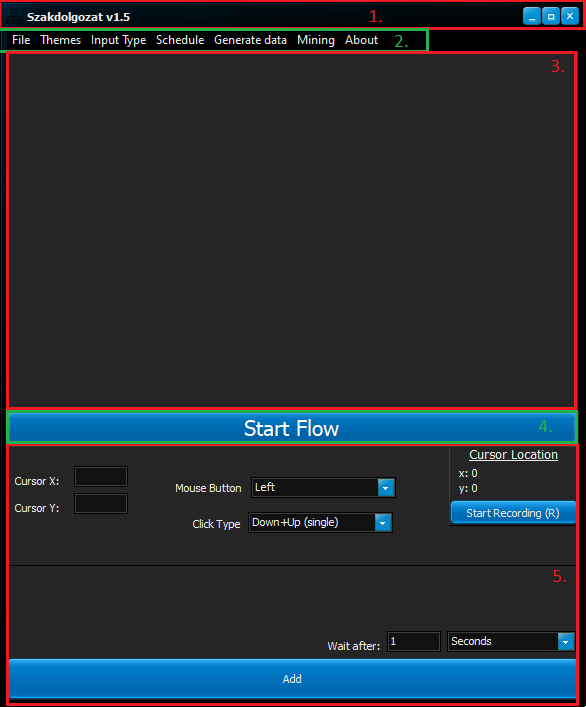
\includegraphics[width=\linewidth, keepaspectratio=true]{images/img_ui_1}	
		\label{fig:ui}
	\end{Figure}
	
	\textbf{Magyarázat}
	\begin{enumerate}
		\item{Fejléc \& rendszer menü}
		\item{Főmenü}
		\item{Folyamati panel}
		\item{Folyamat indító gomb}
		\item{Lépés hozzáadása - egér}
	\end{enumerate}

\end{multicols}

\Section{Főmenü}

Miután a program elindult, a különböző funkciók közötti navigálásra a főmenüt lehet használni. Ennek a használata az alábbiak alapján működik:
\begin{enumerate}
	\item{
		\textbf{File}: Itt van lehetőség a folyamatok külön fájlokként való kezelésére.
		\begin{figure}[h]
			\begin{center}
				\caption{"File" menü}
				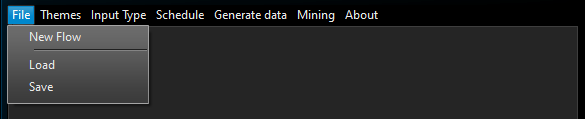
\includegraphics[width=0.5\textwidth, keepaspectratio=true]{images/img_ui_file}\\
				\label{fig:example}
			\end{center}
		\end{figure}

		Lehet: 
		\begin{itemize}
			\item{Új folyamatot létrehozni,}
			\item{Folyamatot fájlból betölteni,}
			\item{Folyamatot lementeni állományba.}
		\end{itemize}
	}
	\item{
		\textbf{Themes}: Ebben a menüben a szoftver felületének a megjelenítését lehet változ\hyp{}tatni. Számos beépített témával rendelkezik amiből választani lehet a felhasználó kedvére.
		\begin{figure}[h]
			\begin{center}
				\caption{"Themes" menü}
				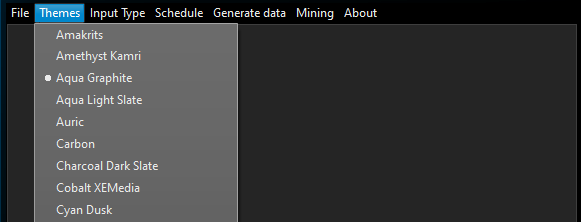
\includegraphics[width=0.5\textwidth, keepaspectratio=true]{images/img_ui_themes}\\
				\label{fig:example}
			\end{center}
		\end{figure}
	}
	\item{
		\textbf{Input Type}: Van lehetőség a jelenlegi folyamathoz kézileg hozzáadni lépést, vagy hozzáfűzni olyan lépéseket amiket a program generál miután rögzítette a felhasználó eseménysorát. Ezeket a funkciókat érjuk el ezzel a menüvel.
		\begin{figure}[h]
			\begin{center}
				\caption{"Input type" menü}
				
\includegraphics[width=0.5\textwidth, keepaspectratio=true]{images/img_ui_input}\\
				\label{fig:example}
			\end{center}
		\end{figure}
		\begin{itemize}
			\item{\textbf{Mouse}: Egérkattintások hozzáadása kézileg}
			\item{\textbf{Keyboard Input}: Billentyű lenyomások hozzáadása kézileg}
			\item{\textbf{Start Recording Input}: Felhasználói eseménysor rögzítése, majd befejezés után lépések generálása.}
		\end{itemize}
	}
	\item{
		\textbf{Schedule}: Itt érhető el a folyamatok időzítésére szolgáló felület.
		\begin{figure}[h!]
			\begin{center}
				\caption{"Schedule" menü}
				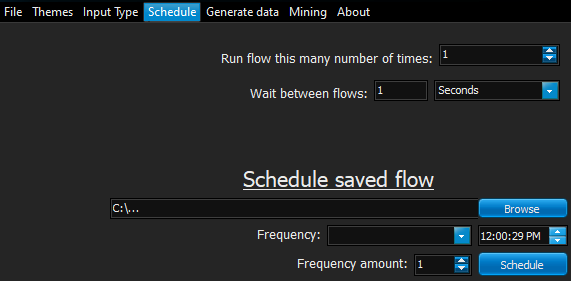
\includegraphics[width=0.3\textwidth, keepaspectratio=true]{images/img_ui_schedule}\\
				\label{fig:example}
			\end{center}
		\end{figure}
	}
	\item{
		\textbf{Generate data}: Folymatokat lehet itt generálni előre meghatározott forgató\hyp{}könyvek alapján.
		\begin{figure}[h!]
			\begin{center}
				\caption{"Generate Data" menü}
				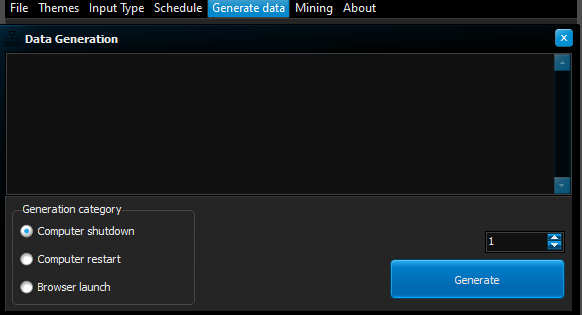
\includegraphics[width=0.5\textwidth, keepaspectratio=true]{images/img_ui_datagen}\\
				\label{fig:example}
			\end{center}
		\end{figure}
	}
	\item{
		\textbf{Mining}: Az adatbányászatra szólgáló felületet itt érjük el.
		\begin{figure}[h!]
			\begin{center}
				\caption{"Mining" menü}
				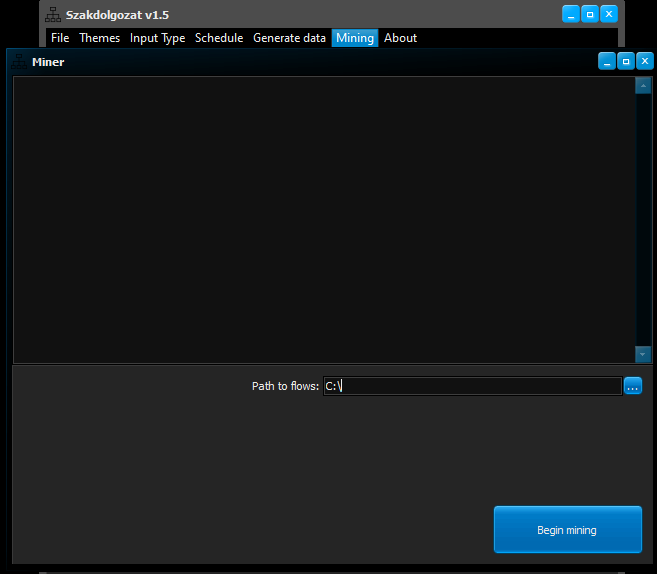
\includegraphics[width=0.5\textwidth, keepaspectratio=true]{images/img_ui_mining}\\
				\label{fig:example}
			\end{center}
		\end{figure}
	}
	\item{
		\textbf{About}: Itt a készítői információ érhető el.
		\begin{figure}[h!]
			\begin{center}
				\caption{"About" menü}
				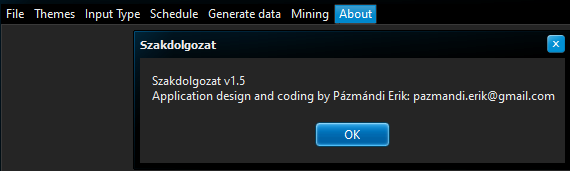
\includegraphics[width=0.5\textwidth, keepaspectratio=true]{images/img_ui_about}\\
				\label{fig:example}
			\end{center}
		\end{figure}
	}

\end{enumerate}

\Section {Folyamathoz tartozó vezérlés}

\Section {Adatbányászat}
\Chapter{Összefoglalás}

ELKÉSZÍTENI (1-2 oldal)

\clearpage

\addcontentsline{toc}{chapter}{Irodalomjegyzék}
\bibliographystyle{apacite}
\bibliography{dolgozat.bib}

\newpage

\pagestyle{empty}

\noindent \textbf{\Large CD Használati útmutató}

\vskip 1cm

\noindent A szakdolgozathoz tartozó CD a következőket tartalmazza:
\begin{enumerate}
\item \textbf{Szoftver futtatható állománya}

Elérési útvonal: \textit{root:/bin/Szakdolgozat.exe}

\item \textbf{Szoftver forráskódja}

Elérési útvonal: \textit{root:/src/}
\item \textbf{Szoftverhez tartozó kiegészítő állományok}

Elérési útvonal: \textit{root:/datamining/}

Bemutató elemezések találhatóak itt, használt előtt egy mappába ki kell csoma\hyp{}golni őket.
\item \textbf{Szakdolgozat dokumentum}

Elérési útvonal: \textit{root:/doc/dolgozat.pdf}
\item \textbf{Szakdolgozat TEX forrás}

Elérési útvonal: \textit{root:/doc/}
\end{enumerate}

A szoftver használatához a CD-ről a számítógépre egy külön könyvtárba szükséges másolni a "Szakdolgozat.exe" fájlt. A folyamatokhoz tartozó bizonyos funkciók (pl. időzítés) csak akkor működnek megfelelően, ha rendszergazdaként futtatjuk, hiszen erre a programra is érvényesek a Windows korlátozásai.



\end{document}
